\chapter{Linearity of Expectation}

\lecture{4}{2 Oct.}{}

So far every probabilistic argument had the same shape: list the bad events, bound the probability of each, and use the union bound to show that with positive probability none of them happens. This chapter replaces probabilities by \emph{expectations}. The basic principle is that a random variable cannot always be above its average, and the tool that makes averages computable is linearity of expectation.

\section{Expectation and the First Moment Principle}\label{sec:first-moment}

Throughout, \((\Omega, \mathbb{P})\) is a probability space and \(X \colon \Omega \to \mathbb{R}\) is a random variable. In all our applications \(\Omega\) is finite, and then the \vocab{expectation} of \(X\) is its weighted average value
\[
    \mathbb{E}[X] = \sum_{\omega \in \Omega} X(\omega) \, \mathbb{P}(\omega).
\]

\subsection{A Random Variable Is Not Always Above Its Mean}

\begin{lemma}[First moment principle]\label{lem:first-moment}
    The events \(\{X \le \mathbb{E}[X]\}\) and \(\{X \ge \mathbb{E}[X]\}\) both have positive probability. In particular
    \[
        \exists\, \omega \in \Omega \text{ s.t.\ } X(\omega) \le \mathbb{E}[X]
        \qquad \text{and} \qquad
        \exists\, \omega' \in \Omega \text{ s.t.\ } X(\omega') \ge \mathbb{E}[X].
    \]
\end{lemma}

\begin{proof}
    Suppose \(\mathbb{P}(X \ge \mathbb{E}[X]) = 0\). Then \(X(\omega) < \mathbb{E}[X]\) for every \(\omega\) with \(\mathbb{P}(\omega) > 0\), and averaging over these \(\omega\) gives
    \[
        \mathbb{E}[X] = \sum_{\omega : \mathbb{P}(\omega) > 0} X(\omega) \, \mathbb{P}(\omega) < \sum_{\omega : \mathbb{P}(\omega) > 0} \mathbb{E}[X] \, \mathbb{P}(\omega) = \mathbb{E}[X],
    \]
    a contradiction. The other event is handled in the same way.
\end{proof}

Think of the values of \(X\) as weights on the real line: \(\mathbb{E}[X]\) is the point where they balance, so there must be weight on each side of it, or on it.
\begin{center}
    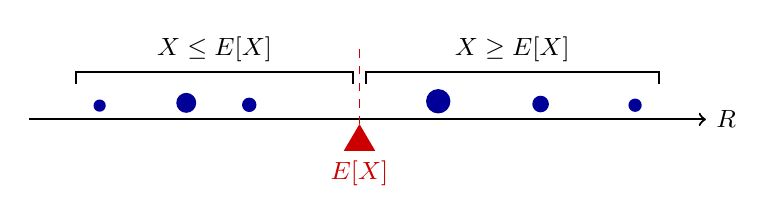
\begin{tikzpicture}[thick, every node/.style={font=\small}]
        \draw[->] (-0.3,0) -- (8.3,0) node[right] {$\mathbb{R}$};
        \foreach \x/\r in {0.6/2.2, 1.7/3.6, 2.5/2.6, 4.9/4.4, 6.2/3.0, 7.4/2.4}
            \fill[blue!60!black] (\x,0.12+\r/40) circle (\r pt);
        \fill[red!80!black] (3.9,-0.06) -- (3.7,-0.4) -- (4.1,-0.4) -- cycle;
        \node[red!80!black, below] at (3.9,-0.4) {$\mathbb{E}[X]$};
        \draw[semithick] (0.3,0.45) -- (0.3,0.6) -- (3.82,0.6) -- (3.82,0.45);
        \node[above] at (2.06,0.6) {$X \le \mathbb{E}[X]$};
        \draw[semithick] (3.98,0.45) -- (3.98,0.6) -- (7.7,0.6) -- (7.7,0.45);
        \node[above] at (5.84,0.6) {$X \ge \mathbb{E}[X]$};
        \draw[red!80!black, dashed, semithick] (3.9,-0.06) -- (3.9,0.9);
    \end{tikzpicture}
\end{center}

This is how we will use it: to show that some object with a property exists, define a random object and a random variable \(X\) measuring the property, compute \(\mathbb{E}[X]\), and conclude that some outcome does at least as well as the average.

\subsection{Linearity}

Computing \(\mathbb{E}[X]\) directly is usually hopeless, since the distribution of \(X\) is complicated. The point is that we never need the distribution: we break \(X\) into simple pieces.

\begin{theorem}[Linearity of expectation]\label{thm:linearity}
    If \(X = \sum_{i=1}^{n} \alpha_i X_i\), where the \(X_i\) are random variables and the \(\alpha_i\) are constants, then
    \[
        \mathbb{E}[X] = \mathbb{E}\Biggl[ \sum_{i=1}^{n} \alpha_i X_i \Biggr] = \sum_{i=1}^{n} \alpha_i \, \mathbb{E}[X_i].
    \]
\end{theorem}

\begin{proof}
    Exchange the two finite sums:
    \[
        \mathbb{E}[X] = \sum_{\omega} \Biggl( \sum_{i=1}^{n} \alpha_i X_i(\omega) \Biggr) \mathbb{P}(\omega)
        = \sum_{i=1}^{n} \alpha_i \sum_{\omega} X_i(\omega) \, \mathbb{P}(\omega)
        = \sum_{i=1}^{n} \alpha_i \, \mathbb{E}[X_i]. \qedhere
    \]
\end{proof}

\begin{remark}
    This holds for \emph{any} random variables \(X_i\); no independence is needed. The proof only ever looks at one outcome \(\omega\) at a time, so it does not care how the \(X_i\) are related to each other. This is what makes linearity so powerful: the pieces \(X_i\) can be as dependent as they like, as in both examples below.
\end{remark}

The pieces we use are almost always indicators.

\begin{definition}[Indicator]
    The \vocab{indicator random variable} of an event \(E\) is
    \[
        \mathbbm{1}_E =
        \begin{cases}
            1, & \text{if } E \text{ occurs}, \\
            0, & \text{otherwise}.
        \end{cases}
    \]
    It satisfies \(\mathbb{E}[\mathbbm{1}_E] = 1 \cdot \mathbb{P}(E) + 0 \cdot \mathbb{P}(E^c) = \mathbb{P}(E)\).
\end{definition}

So if \(X\) counts how many of the events \(E_1, \ldots, E_m\) occur, then \(X = \sum_{i} \mathbbm{1}_{E_i}\), and by \autoref{thm:linearity}
\[
    \mathbb{E}[X] = \sum_{i=1}^{m} \mathbb{E}[\mathbbm{1}_{E_i}] = \sum_{i=1}^{m} \mathbb{P}(E_i).
\]
The expected number of events that occur is the sum of their probabilities, whatever the dependencies between them.

\subsection{Two First Examples}

The first example shows that the union bound arguments of the previous chapter are a special case of the first moment principle.

\begin{eg}[Union bound]\label{eg:union-bound-expectation}
    Let \(E_1, E_2, \ldots, E_m\) be bad events, e.g.\ in Erd\H{o}s's lower bound for \(R(k)\) (\autoref{thm:erdos-ramsey}), the events that a given \(k\)-set of vertices spans a monochromatic clique in a random coloring of \(K_n\). Let
    \[
        X = \#\{\text{bad events that occur}\} = \sum_{i=1}^{m} \mathbbm{1}_{E_i}
        \implies \mathbb{E}[X] = \sum_{i=1}^{m} \mathbb{E}[\mathbbm{1}_{E_i}] = \sum_{i=1}^{m} \mathbb{P}(E_i).
    \]
    If \(\sum_{i} \mathbb{P}(E_i) < 1\), then \(\mathbb{E}[X] < 1\), and by \autoref{lem:first-moment}, with positive probability \(X \le \mathbb{E}[X] < 1\). As \(X\) takes values in \(\{0, 1, 2, \ldots\}\), \(X < 1 \iff X = 0\), i.e.\ with positive probability no bad event occurs. This is exactly the conclusion of the union bound.

    In fact the union bound itself follows. Since \(X\) is a non-negative integer, \(\mathbbm{1}_{\{X \ge 1\}} \le X\) pointwise, and taking expectations,
    \[
        \mathbb{P}\Biggl( \bigcup_{i=1}^{m} E_i \Biggr) = \mathbb{P}(X \ge 1) = \mathbb{E}\bigl[ \mathbbm{1}_{\{X \ge 1\}} \bigr] \le \mathbb{E}[X] = \sum_{i=1}^{m} \mathbb{P}(E_i).
    \]
\end{eg}

\begin{eg}[Fixed points of permutations]\label{eg:fixed-points}
    Let \(\pi \in S_n\) be a uniformly random permutation of \([n]\), and let
    \[
        X(\pi) = \#\{\text{fixed points of } \pi\} = \#\{ i \in [n] : \pi(i) = i \}.
    \]
    \begin{center}
        \begin{tikzpicture}[thick, >={Stealth[length=5pt]}, every node/.style={font=\small}]
            \foreach \i in {1,...,5} {
                \node (t\i) at (1.2*\i,1.3) {$\i$};
                \node (b\i) at (1.2*\i,0) {$\i$};
            }
            \draw[->] (t1) -- (b3);
            \draw[->, red!80!black] (t2) -- (b2);
            \draw[->] (t3) -- (b5);
            \draw[->, red!80!black] (t4) -- (b4);
            \draw[->] (t5) -- (b1);
            \node[anchor=east] at (0.6,1.3) {$i$};
            \node[anchor=east] at (0.6,0) {$\pi(i)$};
            \node[anchor=west, align=left] at (6.8,0.65)
                {\(\pi = \bigl( 3\ 2\ 5\ 4\ 1 \bigr)\)\\fixed points \(2, 4\) in red, \(X(\pi) = 2\)};
        \end{tikzpicture}
    \end{center}
    The distribution of \(X\) is complicated (already \(\mathbb{P}(X = 0)\) needs inclusion--exclusion), but we only want its mean. Write \(X\) as a sum of indicators, one per position:
    \[
        X = \sum_{i=1}^{n} \mathbbm{1}_{\{i \text{ is a fixed point}\}}.
    \]
    For each \(i\), \(\pi(i)\) is uniform on \([n]\), so \(\mathbb{P}(\pi(i) = i) = \frac{(n-1)!}{n!} = \frac{1}{n}\). By linearity,
    \[
        \mathbb{E}[X] = \sum_{i=1}^{n} \mathbb{P}(i \text{ is a fixed point}) = \sum_{i=1}^{n} \frac{1}{n} = 1,
    \]
    for every \(n\). Note that the events \(\{\pi(i) = i\}\) are not independent: if \(n - 1\) of them occur, so does the last one. Linearity does not notice.
\end{eg}

\section{Sum-Free Sets}\label{sec:sum-free}

The first real application of the first moment principle is to a problem in additive combinatorics.

\subsection{The Problem}

\begin{definition}[Sum-free set]\label{def:sum-free}
    A \vocab{sum} is a triple of integers \((x, y, z)\) s.t.\ \(x + y = z\). A set \(A \subseteq \mathbb{Z}\) is \vocab{sum-free} if there is no sum in \(A^3\), i.e.\ there are no \(x, y, z \in A\) with \(x + y = z\).
\end{definition}

Here \(x, y, z\) need not be distinct: a sum-free set cannot contain both \(x\) and \(2x\), and it never contains \(0 = 0 + 0\). The same definition makes sense in any abelian group, and we will use it in \(\mathbb{Z}_p\).

\begin{definition}
    Given a finite set \(S \subseteq \mathbb{Z}\), let
    \[
        f(S) = \max\{ \abs{A} : A \subseteq S \text{ is sum-free} \}
    \]
    be the size of a largest sum-free subset of \(S\).
\end{definition}

\begin{eg}[{Warm-up: \(f([n]) = \lceil \frac{n}{2} \rceil\)}]\label{eg:sum-free-interval}
    \emph{Lower bound.} Two sum-free subsets of \([n]\) of size \(\lceil \frac{n}{2} \rceil\) are
    \begin{itemize}
        \item the odd numbers, since odd \(+\) odd is even;
        \item the numbers \(> \frac{n}{2}\), since the sum of two of them exceeds \(n\) and so is not in the set.
    \end{itemize}
    \begin{center}
        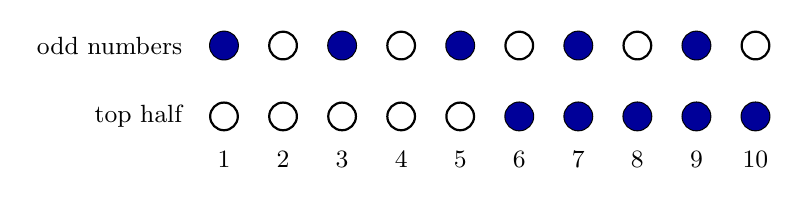
\begin{tikzpicture}[thick, every node/.style={font=\small}]
            \foreach \row/\lab in {0/{odd numbers}, -0.9/{top half}} {
                \foreach \i in {1,...,10} \draw (0.75*\i,\row) circle (5pt);
                \node[anchor=east] at (0.35,\row) {\lab};
            }
            \foreach \i in {1,3,5,7,9} \fill[blue!60!black] (0.75*\i,0) circle (5pt);
            \foreach \i in {6,...,10} \fill[blue!60!black] (0.75*\i,-0.9) circle (5pt);
            \foreach \i in {1,...,10} \node at (0.75*\i,-1.45) {$\i$};
        \end{tikzpicture}
    \end{center}
    \emph{Upper bound.} Let \(A \subseteq [n]\) be sum-free and \(a = \max A\). For every \(x < a\), at most one of \(x\) and \(a - x\) lies in \(A\), since \(x + (a - x) = a \in A\). The pairs \(\{x, a - x\}\) cover \([a-1]\):
    \begin{center}
        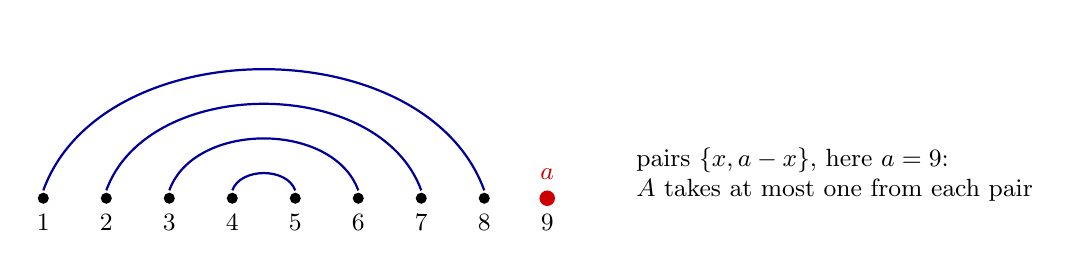
\begin{tikzpicture}[thick, every node/.style={font=\small}]
            \foreach \i in {1,...,9} \fill (0.8*\i,0) circle (2pt) node[below=2pt] {$\i$};
            \foreach \i in {1,...,4} {
                \pgfmathtruncatemacro{\j}{9-\i}
                \draw[blue!60!black] (0.8*\i,0.1) to[out=70, in=110] (0.8*\j,0.1);
            }
            \fill[red!80!black] (0.8*9,0) circle (2.8pt);
            \node[red!80!black, above=3pt] at (0.8*9,0) {$a$};
            \node[anchor=west, align=left] at (8.2,0.3)
                {pairs \(\{x, a - x\}\), here \(a = 9\):\\\(A\) takes at most one from each pair};
        \end{tikzpicture}
    \end{center}
    If \(a\) is odd there are \(\frac{a-1}{2}\) pairs, so \(\abs{A} \le \frac{a-1}{2} + 1 = \frac{a+1}{2}\). If \(a\) is even there are \(\frac{a-2}{2}\) pairs and the middle element \(\frac{a}{2}\) is excluded on its own, as \(\frac{a}{2} + \frac{a}{2} = a\), so \(\abs{A} \le \frac{a-2}{2} + 1 = \frac{a}{2}\). Either way \(\abs{A} \le \frac{a+1}{2} \le \frac{n+1}{2}\), i.e.\ \(\abs{A} \le \lceil \frac{n}{2} \rceil\).
\end{eg}

So an interval always contains a sum-free half. The interval is very structured, though, and both constructions used that structure. What if the numbers are arbitrary?

\begin{question}
    Does \emph{every} set of \(n\) integers contain a large sum-free subset?
\end{question}

\begin{definition}
    For \(n \in \mathbb{N}\), let\footnote{We exclude \(0\), which can never lie in a sum-free set.}
    \[
        f(n) = \min\{ f(S) : S \subseteq \mathbb{Z} \setminus \{0\},\ \abs{S} = n \}.
    \]
\end{definition}

\begin{remark}[Why the minimum]
    The maximum is trivially \(n\): take \(S\) itself sum-free, e.g.\ \(a,\ b > 2a,\ 2b + 1,\ 4b + 3, \ldots\) with \(a > 0\), each element larger than twice the previous one, hence not a sum of two earlier ones.\footnote{\(x = y\) is allowed, so beating \(a + b\) is not enough: \(1 + 1 = 2\).}
\end{remark}

\begin{observation}
    \(f(n) \le f([n]) = \lceil \frac{n}{2} \rceil\).
\end{observation}

Now \(S\) may be any set of non-zero integers, including negative ones, with no structure to exploit. Yet a constant fraction of it can always be kept.

\begin{theorem}[Erd\H{o}s, 1965]\label{thm:sum-free}
    \(f(n) \ge \frac{n+1}{3}\). That is, every set of \(n\) non-zero integers contains a sum-free subset of size at least \(\frac{n+1}{3}\).
\end{theorem}

\begin{proof}
    Let \(S \subseteq \mathbb{Z} \setminus \{0\}\) with \(\abs{S} = n\).

    \begin{lemma}\label{lem:primes-2-mod-3}
        There are infinitely many primes \(p \equiv 2 \pmod 3\).
    \end{lemma}
    \begin{subproof}
        Given such primes \(p_1, \ldots, p_m\), let \(N = 3 p_1 \cdots p_m - 1 \equiv 2 \pmod 3\). Then \(3 \nmid N\), and not all prime factors of \(N\) are \(\equiv 1 \pmod 3\), else \(N \equiv 1\). So some prime \(q \equiv 2 \pmod 3\) divides \(N\), and \(q \ne p_i\) since \(p_i \mid N + 1\).
    \end{subproof}

    By \autoref{lem:primes-2-mod-3}, choose a prime \(p = 3k + 2\) with \(p > \max_{s \in S} \abs{s}\), so \(p \nmid s\) for all \(s \in S\). We identify \(\mathbb{Z}_p\) with \(\{0, 1, \ldots, p-1\}\), and for an integer \(m\) write \(m \bmod p \in \{0, 1, \ldots, p-1\}\) for its remainder. Let
    \[
        C = \{k+1, k+2, \ldots, 2k+1\}.
    \]

    \begin{lemma}\label{lem:middle-third}
        \(C\) is sum-free in \(\mathbb{Z}_p\), and \(\dfrac{\abs{C}}{p - 1} = \dfrac{k+1}{3k+1} > \dfrac{1}{3}\).
    \end{lemma}
    \begin{subproof}
        For \(c_1, c_2 \in C\) we have \(2k+2 \le c_1 + c_2 \le 4k+2\). If \(c_1 + c_2 \le 3k+1\), then \((c_1 + c_2) \bmod p = c_1 + c_2 \in R = \{2k+2, \ldots, 3k+1\}\); otherwise \((c_1 + c_2) \bmod p = c_1 + c_2 - p \in L = \{0, \ldots, k\}\). Either way \((c_1 + c_2) \bmod p \notin C\). Finally \(\abs{C} = k+1\) and \(p - 1 = 3k+1\).
    \end{subproof}
    \begin{center}
        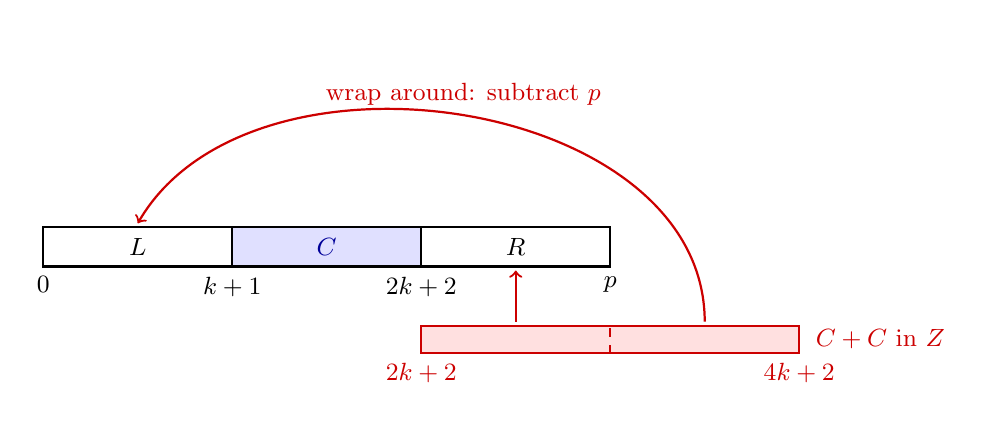
\begin{tikzpicture}[x=0.8cm, thick, every node/.style={font=\small}]
            \fill[blue!12] (3,-0.25) rectangle (6,0.25);
            \draw (0,-0.25) rectangle (9,0.25);
            \draw (3,-0.25) -- (3,0.25);
            \draw (6,-0.25) -- (6,0.25);
            \node at (1.5,0) {$L$};
            \node[blue!60!black] at (4.5,0) {$C$};
            \node at (7.5,0) {$R$};
            \node[below] at (0,-0.25) {$0$};
            \node[below] at (3,-0.25) {$k+1$};
            \node[below] at (6,-0.25) {$2k+2$};
            \node[below] at (9,-0.25) {$p$};
            % C + C as integers: from 2k+2 to 4k+2, overshooting p
            \fill[red!12] (6,-1.35) rectangle (12,-1.0);
            \draw[red!80!black] (6,-1.35) rectangle (12,-1.0);
            \draw[red!80!black, dashed] (9,-1.35) -- (9,-1.0);
            \node[red!80!black, anchor=west] at (12.1,-1.175) {$C + C$ in $\mathbb{Z}$};
            \node[red!80!black, below] at (6,-1.35) {$2k+2$};
            \node[red!80!black, below] at (12,-1.35) {$4k+2$};
            % the part beyond p wraps back onto L
            \draw[->, red!80!black] (10.5,-0.95) to[out=90, in=60] node[pos=0.5, above] {wrap around: subtract $p$} (1.5,0.3);
            \draw[->, red!80!black] (7.5,-0.95) -- (7.5,-0.3);
        \end{tikzpicture}
    \end{center}

    Let \(x\) be uniformly random in \(\{1, 2, \ldots, p-1\}\), i.e.\ \(\mathbb{P}(x = a) = \frac{1}{p-1}\) for each \(a\), and
    \[
        A_x = \{ s \in S : xs \bmod p \in C \} \subseteq S.
    \]
    We show that every \(A_x\) is sum-free, and that \(\abs{A_x} \ge \frac{n+1}{3}\) for some \(x\); this \(A_x\) then proves the theorem.

    \(A_x\) is sum-free: if \(s_1 + s_2 = s_3\) with \(s_1, s_2, s_3 \in A_x\), then \(x s_1 + x s_2 = x s_3\), so \((x s_1 \bmod p) + (x s_2 \bmod p) \equiv x s_3 \bmod p \pmod p\) with all three remainders in \(C\), contradicting \autoref{lem:middle-third}.

    Fix \(s \in S\). We claim that \(xs \bmod p\) takes each value \(1, 2, \ldots, p-1\) with probability exactly \(\frac{1}{p-1}\). Consider
    \[
        \varphi_s \colon \{1, \ldots, p-1\} \to \{1, \ldots, p-1\}, \qquad a \mapsto as \bmod p.
    \]
    \begin{itemize}
        \item It is well defined, i.e.\ \(as \bmod p \ne 0\): \(p\) is prime and \(p \nmid a\), \(p \nmid s\), so \(p \nmid as\).
        \item It is injective: if \(as \bmod p = a's \bmod p\), then \(p \mid (a - a')s\), so \(p \mid a - a'\) as \(p \nmid s\); since \(\abs{a - a'} < p\), \(a = a'\).
        \item An injection of a finite set into itself is a bijection.
    \end{itemize}
    So for each \(y \in \{1, \ldots, p-1\}\) there is exactly one \(a\) with \(as \bmod p = y\), and
    \[
        \mathbb{P}(xs \bmod p = y) = \mathbb{P}(x = \varphi_s^{-1}(y)) = \frac{1}{p-1}.
    \]
    Summing over \(y \in C\),
    \[
        \mathbb{P}(xs \bmod p \in C) = \sum_{y \in C} \frac{1}{p-1} = \frac{\abs{C}}{p-1} = \frac{k+1}{3k+1} > \frac{1}{3}.
    \]
    Writing \(\abs{A_x} = \sum_{s \in S} \mathbbm{1}_{\{xs \bmod p \in C\}}\), linearity of expectation gives
    \[
        \mathbb{E}\bigl[ \abs{A_x} \bigr] = \sum_{s \in S} \mathbb{P}(xs \bmod p \in C) > \frac{n}{3}.
    \]
    By \autoref{lem:first-moment} some \(x\) has \(\abs{A_x} > \frac{n}{3}\), and as \(\abs{A_x}\) is an integer, \(\abs{A_x} \ge \frac{n+1}{3}\).
\end{proof}

\begin{remark}
    So \(\frac{n+1}{3} \le f(n) \le \lceil \frac{n}{2} \rceil\). Bourgain (1997) improved the lower bound to \(\frac{n+2}{3}\), and Eberhard, Green and Manners (2014) showed that the constant \(\frac{1}{3}\) cannot be improved: \(f(n) \le \bigl( \frac{1}{3} + o(1) \bigr) n\). So for arbitrary sets the random dilation is essentially optimal, and the interval \([n]\), with its sum-free half, is far from the worst case.
\end{remark}
